\index{système!ouvert|(textbf}
\section{Pourquoi utiliser un système ouvert ?}
\index{système!fermé, utilité de}\index{système!ouvert, utilité de}\index{système!fermé vs. ouvert}

	Dans de nombreuses machines, le fluide utilisé pour transférer de la chaleur et du travail circule de façon continue. Il peut alors être difficile d’identifier une quantité de masse fixe pour en faire un système fermé et y quantifier les transferts d’énergie. Par exemple, dans une tuyère de turboréacteur, l’air se détend et accélère continûment : à un instant donné il n’y a pas de volume identifiable qui aurait \emph{une} vitesse ou \emph{une} pression particulière.
	
	L’emploi d’un système ouvert nous est très utile pour comptabiliser l’énergie dans les flux. Plutôt que de séparer les étapes dans le temps (par exemple avant et après une compression) nous allons quantifier les transferts de travail et de chaleur en séparant les étapes dans l’espace (par exemple en amont et en aval du compresseur).

\section{Conventions de comptabilité}
\label{ch_conventions_compta_so}

	\subsection{Le système ouvert}
	\label{ch_convention_signe_so}
	\index{système!fermé, conventions de signe}

		\thermoquotebegin{O}
			Les difficultés de construction qui doivent être surmontées dans un moteur à gaz puissant, à cause des pressions énormes sur les pistons et de la dilatation des culasses (gare aux fissures !) sont bien connues. Une turbine à gaz sûre serait, de ce point de vue, une amélioration.
		\thermoquoteend{Aurel Stodola, 1904}{\textit{Die Dampfturbinen}~\cite{stodola1904, stodola1905}\vspace{3em}\index{Stodola!Aurel}} %handmade vspace
		Nous appelons \vocab[système!ouvert, définition]{système ouvert} un sujet d’étude arbitraire dont les frontières sont perméables à la masse (\cref{fig_systeme_ouvert}). En général, son volume peut changer, et il peut posséder plusieurs entrées et sorties, chacune avec un débit et une pression différents.

		\onlyframabook{\begin{figure}}
		\onlyamphibook{\begin{figure}[htc]}%handmade pour poser la figure
			\begin{center}
				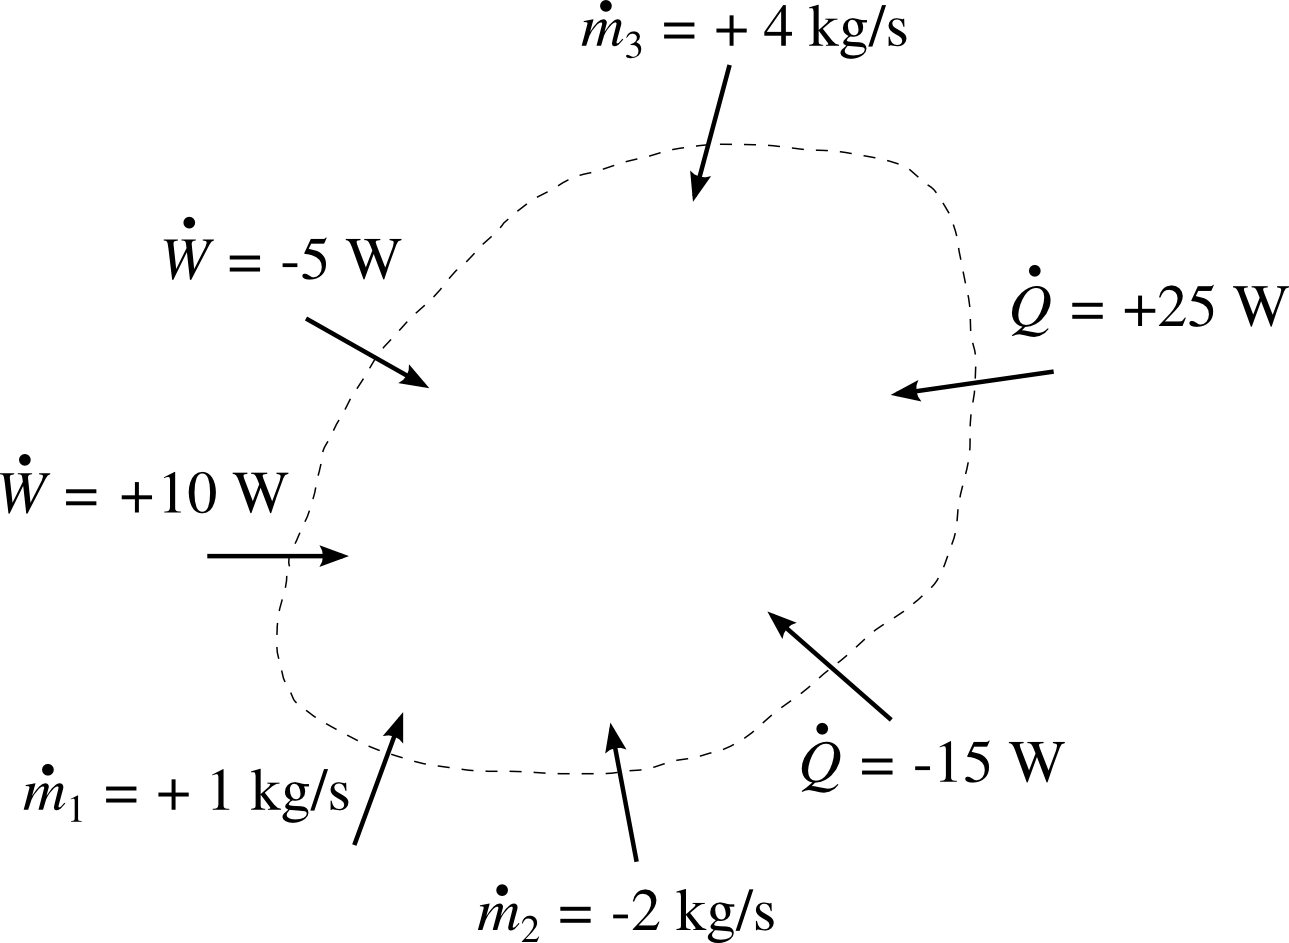
\includegraphics[width=8cm]{images/convention_systeme_ouvert.png}
			\end{center}
			\supercaption{Conventions de signe pour un système ouvert. Les flux entrants sont positifs, les flux sortants sont négatifs ; ils sont tous représentés avec des flèches rentrantes.}{schéma \cczero \oc}
			\label{fig_systeme_ouvert}
		\end{figure}

		Dans notre étude de la thermodynamique, nous n’allons utiliser que des systèmes ouverts :
		\begin{itemize}
			\item de volume fixe ;
			\item ne possédant qu’une seule entrée et qu’une seule sortie ;
			\item traversés par un débit de masse $\dot m$ constant (positif par convention).
		\end{itemize}
		Ces systèmes sont dits en \vocab[regime@régime continu]{régime continu}\footnote{On dit aussi parfois \vocab[]{régime permanent} ou \vocab[]{stationnaire}.\index{continu, régime}}.

	\dontbreakpage %handmade, pour éviter un drôle de saut de page
	\subsection{Conventions de signe}
	\index{système!fermé, conventions de signe}

		Tout comme pour les systèmes ouverts, nous allons nous placer du point de vue du système pour quantifier les transferts :
			\begin{itemize}
				\item La réception de travail, de chaleur ou de masse se traduit par un transfert~\emph{positif} ;
				\item La perte de travail, de chaleur ou de masse se traduit par un transfert \emph{négatif}.
			\end{itemize}
		
		Nous additionnons donc tous les transferts comme sur un relevé de compte en banque.


\section{Le premier principe dans un système ouvert}
\index{système!ouvert, premier principe}\index{principes de la thermodynamique!premier, système ouvert}

	Nous avons vu que dans un système fermé le principe de conservation de l’énergie se traduisait par l’expression $q + w = \Delta u$ (\ref{eq_premier_principe_sf_maj}). Dans un système ouvert, la situation est un peu différente et nous devons tenir compte d’autres formes d’énergie.

	\subsection{Entrer et sortir du système : le travail d’écoulement}
	\index{travail!d’écoulement}\index{travail!d’insertion}\index{travail!d’extraction}

		Imaginons un système ouvert en régime continu contenant une petite pompe à eau. Pour insérer l’eau dans la pompe à une pression donnée, il faut fournir de l’énergie au système. Au contraire, pour repousser l’eau à l’extérieur (à une pression plus haute), le système doit fournir de l’énergie. Comment quantifier cette énergie ?

		Considérons le cas d’un \vocab[element@élément de fluide]{élément de fluide}\index{fluide, élément de} (c’est-à-dire une petite quantité de fluide en transit, de volume $V_\text{élément}$) qui pénètre à l’intérieur de notre système à la pression $p_1$ (\cref{fig_travail_ecoulement}).

		\begin{figure}
			\begin{center}
				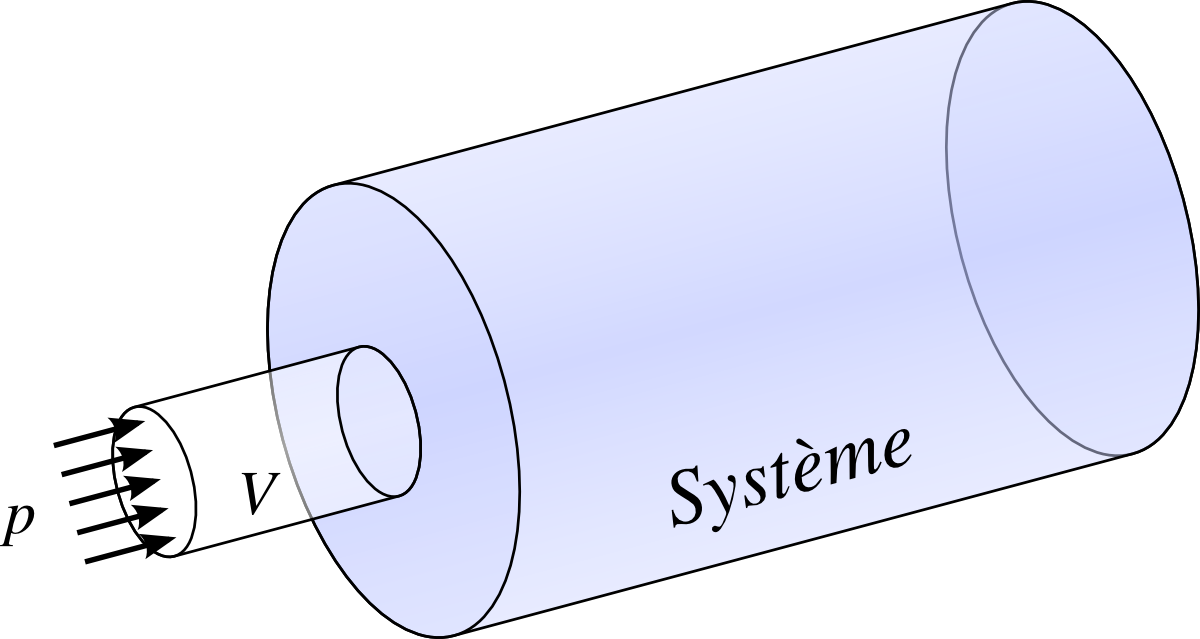
\includegraphics[width=8cm]{images/travail_insertion.png}
			\end{center}
			\supercaption{Un élément de fluide de volume $V_\text{élément}$ pénétrant à la pression~$p$ dans le système ouvert.}{schéma \cczero \oc}
			\label{fig_travail_ecoulement}
		\end{figure}

		Le travail $W_\text{insertion}$ reçu par le système lorsque l’élément est poussé à travers l’insertion est :
		\begin{IEEEeqnarray}{rCl}
			W_\text{insertion} 	& = & p_1 \ V_\text{élément}
		\end{IEEEeqnarray}
		\begin{equationterms}
			\item où \tab $W_\text{insertion}$ 	\tab est le travail d’insertion (\si{\joule}),
			\item et \tab $V_\text{élément}$ 	\tab\tab\tab est le volume de l’élément de fluide (\si{\metre\cubed}).
		\end{equationterms}

		Si un tel volume de fluide pénètre chaque seconde dans le système, alors ce dernier reçoit une puissance sous forme de travail, que nous nommons \vocab[puissance!d’insertion]{puissance d’insertion}, $\dot{W}_\text{insertion}$. Nous l’exprimons parfois sous forme spécifique~(\S\ref{ch_valeurs_spécifiques}) :
		\begin{IEEEeqnarray}{rCl}
			\dot{W}_\text{insertion} 	& = & p_1 \ \dot{V}_1 = \dot m_1 \ p_1 \ v_1 = \dot m \ p_1 \ v_1\\
			w_\text{insertion} 			& = & p_1 \ v_1
			\label{eq_puissance_spé_insertion}	
		\end{IEEEeqnarray}
		\begin{equationterms}
			\item où \tab $\dot{W}_\text{insertion}$ 	\tab est la puissance d’insertion (\si{\watt}),
			\item 	\tab $w_\text{insertion}$ 			\tab\tab est la puissance spécifique d’insertion (\si{\joule\per\kilogram}),
			\item		\tab $\dot m_1$ 	est le débit net de masse en 1 (\si{\kilogram\per\second}),
			\item		\tab $\dot m$ 		\tab est le débit de masse traversant le système (toujours positif, \si{\kilogram\per\second}),
			\item 	\tab $\dot{V}_1$ 	\tab est le débit volumique de fluide (\si{\metre\cubed\per\second})
			\item et \tab $v_1$ 			\tab est le volume spécifique du fluide à l’entrée (\si{\metre\cubed\per\kilogram}).
		\end{equationterms}

		De la même façon, pour que le fluide sorte du système à son autre extrémité, il faut que le système fournisse continûment une puissance nommée \vocab[puissance!d’extraction]{puissance d’extraction} :
		\begin{IEEEeqnarray}{rCl}
			\dot{W}_\text{extraction} 	& = & - p_2 \ \dot{V_2} = \dot{m}_2 \ p_2 \ v_2 = - \dot{m} \ p_2 \ v_2 \\
			w_\text{extraction} 			& = & - p_2 \ v_2
		\end{IEEEeqnarray}
		\begin{equationterms}
			\item où le débit sortant $\dot m_2$ (négatif) est exprimé en fonction du débit $\dot m$ traversant le système (toujours positif, \si{\kilogram\per\second}).
		\end{equationterms}

		La somme nette de ces deux puissances aux frontières est nommée \vocab[puissance!d’écoulement]{puissance d’écoulement}, $\dot{W}_\text{écoulement} \equiv \dot{W}_\text{insertion} + \dot{W}_\text{extraction}$ . Son signe dépend des conditions d’opération -- l’étudiant/e est encouragé/e à se représenter et à formuler les conditions dans lesquelles la puissance d’écoulement peut être négative, nulle, ou positive.


	\subsection{Bilan énergétique}

		Essayons de concevoir un système ouvert en régime continu de la façon la plus générale possible, comme représenté en \cref{fig_système_ouvert}. Nous allons maintenant y comptabiliser tous les transferts d’énergie.

		\begin{figure}
			\begin{center}
				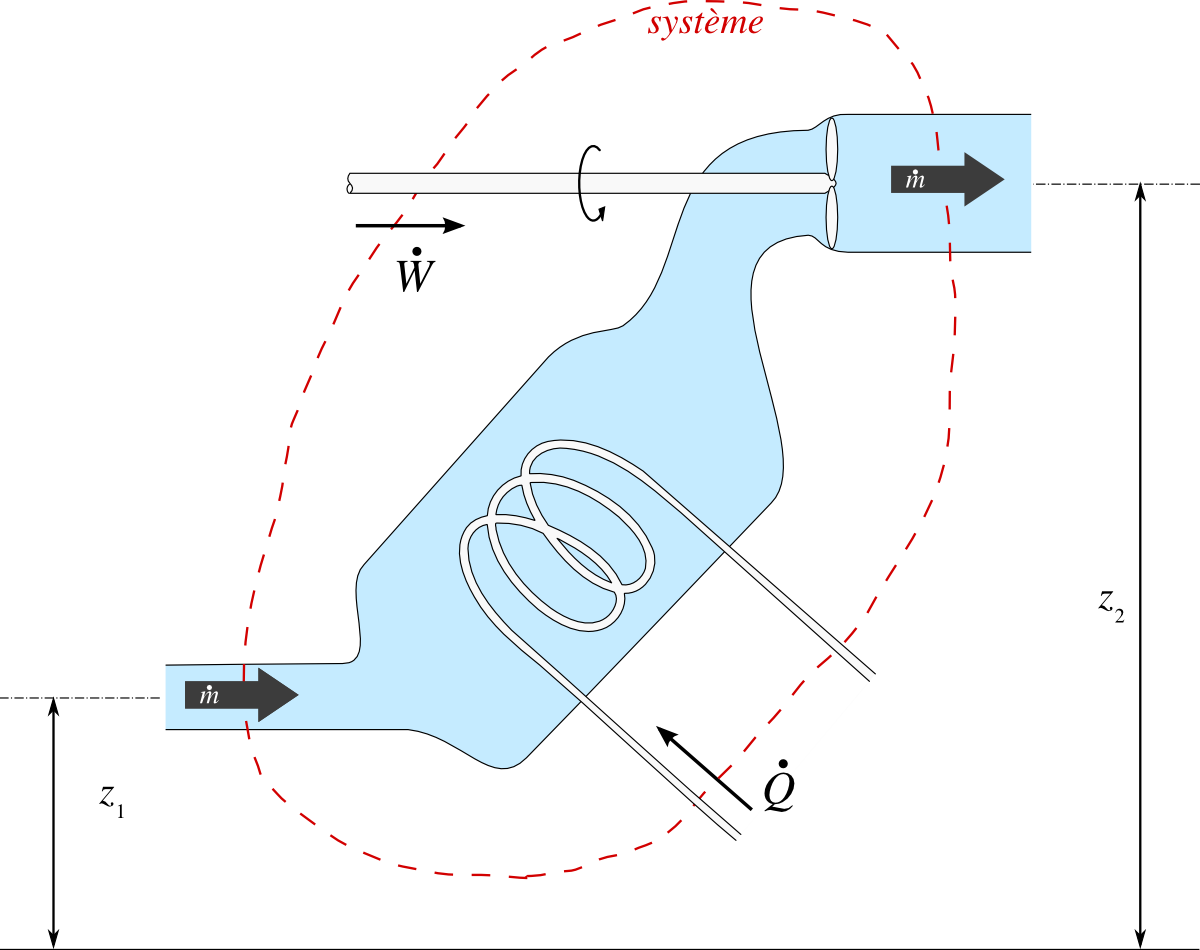
\includegraphics[width=\textwidth]{images/sfee.png}
			\end{center}
			\supercaption{Système ouvert arbitraire. Le système (dont les frontières sont en pointillés, en rouge) est traversé de gauche à droite par le fluide qui circule avec un débit de masse $\dot{m}$ constant. Il reçoit une puissance $\dot{W}_{1 \to 2}$ sous forme de travail et une puissance $\dot{Q}_{1 \to 2}$ sous forme de chaleur.}{schéma \cczero \oc}
			\label{fig_système_ouvert}
		\end{figure}

		Lorsqu’il pénètre dans le système, le fluide possède déjà une énergie interne~$u_1$ ; le système voit donc son énergie interne augmenter avec la puissance $\dot{U}_{1}$ :
		\begin{equation}
			\dot{U}_{1} = \dot{m} \ u_1
			\label{eq_w_int1}
		\end{equation}

		De même, le fluide possède une quantité d’énergie mécanique spécifique $e_\text{méca1}$ (\ref{def_énergie_mécanique_spécifique}) et le système reçoit donc également une puissance $\dot{E}_\text{méca1}$ :
		\begin{equation}
			\dot{E}_\text{méca1} = \dot m \ e_\text{méca1} = \dot{m} \ \left(\frac{1}{2} \ C_1^2 + g \ z_1\right)
			\label{eq_w_méc1}
		\end{equation}

		Ces expressions~\ref{eq_w_int1} et~\ref{eq_w_méc1} sont de signe opposé à la sortie du système, où nous leur attribuons l’indice~2.
		
		Nous avons donc fait le tour des formes d’énergie que l’on peut observer dans un système ouvert : travail d’écoulement, énergie interne, et énergie mécanique. Puisque le premier principe stipule que l’énergie est indestructible (\S\ref{ch_premier_principe}), l’ajout d’une puissance $\dot Q$ sous forme de chaleur ou $\dot W$ sous forme de travail ne peut faire varier que ces trois formes-là. Cela se traduit par l’équation :
		\begin{IEEEeqnarray}{rCl}
			\dot{Q}_{1 \to 2} + \dot{W}_{1 \to 2} + \left(\dot{W}_\text{insertion} + \dot{U}_{1} + \dot{E}_\text{méca1}\right) + \left(\dot{W}_\text{extraction} + \dot{U}_{2} + \dot{E}_\text{méca2}\right) = 0	\nonumber\\
			\label{eq_somme_puissances}
		\end{IEEEeqnarray}
		\begin{equationterms}
			\item où tous les termes sont exprimés en \si{watts}.
		\end{equationterms}

		Nous pouvons ré-exprimer l’\cref{eq_somme_puissances} en fonction de grandeurs directement mesurables :
		\begin{IEEEeqnarray}{rCl}
			\dot{Q}_{1 \to 2} + \dot{W}_{1 \to 2}  + \dot{m} \ \left(p_1 \ v_1 + u_1 + \frac{1}{2} C_1^2 + g \ z_1\right) &=& \dot{m} \ \left(p_2 \ v_2 + u_2 + \frac{1}{2} C_2^2 + g \ z_2\right)\nonumber\\
			\label{eq_grande_sfee}
		\end{IEEEeqnarray}
		ou encore :
		\begin{IEEEeqnarray}{rCl}
			\dot{Q}_{1 \to 2} + \dot{W}_{1 \to 2} 	& = & \dot{m} \left[ \Delta u + \Delta (p v) + \frac{1}{2} \Delta \left(C^2\right) + g \ \Delta z \right] 	\label{eq_grande_sfee_deltas} \\
			q_{1 \to 2} + w_{1 \to 2} 		& = & \Delta u + \Delta (p v) + \Delta e_\text{méca.}  \label{eq_petite_sfee_deltas}
		\end{IEEEeqnarray}
		\begin{equationterms}
			\item où les symboles $\Delta$ indiquent la variation des propriétés entre les points~1 et~2 du système.
		\end{equationterms}
		
		Les équations~\ref{eq_grande_sfee} et~\ref{eq_petite_sfee_deltas} sont extrêmement utiles en thermodynamique, puisqu’elles permettent de quantifier par déduction les puissances en jeu dans les écoulements. Elles nous permettent notamment de prédire les propriétés du fluide à la sortie d’un dispositif dont on connaît la puissance mécanique et les émissions de chaleur. Par exemple, on peut connaître l’énergie restante dans l’air à la sortie d’une turbine dont on connaît la puissance.
		
		\begin{anexample}
			Un compresseur de turboréacteur admet \SI{1,5}{\kilogram\per\second} d’air à une pression de~\SI{0,8}{\bar}, énergie interne de~\SI{192,5}{\kilo\joule\per\kilogram} et volume spécifique de~\SI{0,96}{\metre\cubed\per\kilogram}. Il compresse l’air jusqu’à \SI{30}{\bar}, le restituant avec une énergie interne de~\SI{542,3}{\kilo\joule\per\kilogram} et un volume spécifique de~\SI{6,19e-2}{\metre\cubed\per\kilogram}. La vitesse et l’altitude de l’air sont inchangés.
			
			Quelle est la puissance du compresseur, si ses transferts de chaleur sont négligeables ?
				\begin{answer}
					Nous appliquons l’\cref{eq_grande_sfee_deltas} pour obtenir :  $\dot{W}_{1 \to 2}
					= -\dot{Q}_{1 \to 2} + \dot{m} \left[ \Delta u + \Delta (p v) + \frac{1}{2} \Delta \left(C^2\right) + g \ \Delta z \right]
					= 0 + \dot{m} \left[ \Delta u + \Delta (p v) + 0 + 0 \right]
					= \num{1,5} \left[ (\num{542,3e3} - \num{192,5e3}) + (\num{30e5}\times\num{6,19e-2} - \num{0,8e5}\times\num{0,96})\right]
					= \SI{+6,881e5}{\watt} = \SI{+688,1}{\kilo\watt}$.
					\begin{remark}La seule difficulté dans l’application de cette équation concerne la bonne conversion des unités. Il faut toujours convertir les pressions et énergies depuis leurs unités usuelles vers des unités \textsc{si}.\end{remark}
					\begin{remark}La puissance est positive, ce qui ne nous surprend pas puisque l’air \emph{reçoit} le travail. Dans une turbine, le travail serait négatif.\end{remark}
				\end{answer}
		\end{anexample}

	\subsection{L’enthalpie}

		Dans de très nombreux cas, les termes $u$ et $p v$ varient de la même façon avec l’état du fluide%
			\footnote{Nous verrons dans le prochain chapitre que dans le cas d’un gaz parfait, ils sont tous deux proportionnels à la température.}%
		. Pour simplifier leur utilisation dans les calculs, ils sont souvent regroupés en un seul terme.

		Nous nommons la somme des termes $u$ et $p v$ l’\vocab[enthalpie!spécifique]{enthalpie spécifique}\index{spécifique!enthalpie}, et lui attribuons le symbole~$h$ :
		\begin{equation}
			h \equiv u + p \ v
			\label{def_enthalpie}
		\end{equation}
		\begin{equationterms}
			\item où les termes sont exprimés en \si{\joule\per\kilogram}.
		\end{equationterms}

		Bien sûr, l’\vocab[enthalpie!définition|textbf]{enthalpie} $H$ se définit simplement comme :
		\begin{equation}
			H \equiv m \ h
		\end{equation}
		\begin{equationterms}
		      \item où \tab $H$ \tab est mesurée en \si{joules} (\si{\joule}).
		\end{equationterms}

		\thermoquotebegin{O}
			La diminution de la teneur en chaleur est égale à la valeur équivalente en chaleur du “travail utile” reçu, plus la chaleur transmise à l’extérieur plus l’augmentation en énergie cinétique par kilogramme de vapeur.
		\thermoquoteend{Aurel Stodola, 1904\\{\tiny(où la «~teneur en chaleur~» $\lambda$ n’est pas encore nommée \textit{enthalpie})}}{\textit{Die Dampfturbinen}~\cite{stodola1904, stodola1905}\vspace{1em}\index{Stodola!Aurel}} %handmade vspace
		En pratique, le terme \textit{enthalpie} est souvent utilisé même s’il s’agit d’enthalpie massique ; le symbole et le contexte permettent de préciser de quelle variable il s’agit.

		En faisant usage du concept d’enthalpie, les équations~\ref{eq_grande_sfee} et~\ref{eq_petite_sfee_deltas} s’allègent pour devenir :
		\begin{IEEEeqnarray}{rCl}
			\dot{Q}_{1 \to 2} + \dot{W}_{1 \to 2} 	& = & \dot{m} \left( \Delta h + \Delta e_\text{méca.} \right) \label{eq_grande_sfee_deltas_h} \\
			q_{1 \to 2} + w_{1 \to 2} 		& = & \Delta h + \Delta e_\text{méca.}	\label{eq_petite_sfee_deltas_h}
		\end{IEEEeqnarray}

		Nous voyons ainsi que dans un système ouvert, les transferts de chaleur et de travail font varier \emph{l’enthalpie} du fluide, et non seulement son énergie interne comme dans un système fermé.

		\begin{anexample}	
			Dans une tuyère, l’air est détendu sans transfert de travail ni de chaleur. Il entre avec une enthalpie spécifique de~\SI{776}{\kilo\joule\per\kilogram} et une vitesse de~\SI[per-mode = symbol]{30}{\kilo\metre\per\hour} et ressort à même altitude, avec une enthalpie de~\SI{636}{\kilo\joule\per\kilogram}.
			
			Quelle est la vitesse d’éjection de l’air ?
				\begin{answer}
					Nous partons de l’équation~\ref{eq_petite_sfee_deltas_h} :
						\begin{IEEEeqnarray*}{rCl}
							q_{1 \to 2} + w_{1 \to 2} 		& = & \Delta h + \Delta e_\text{méca.}\\
							\Delta e_\text{méca.} 			& = & -\Delta h - 0 - 0 \\
							\frac{1}{2}\left(C_2^2 - C_1^2\right) & = & - \Delta h\\
							C_2 &=& \left[ -2 \ \Delta h + C_1^2\right]^{\frac{1}{2}}
						\end{IEEEeqnarray*}
					Ainsi $C_2 = \left[-2\times(\num{636e3} - \num{776e3}) + \left(\frac{30}{\num{3,6}}\right)^2 \right]^{\frac{1}{2}}
						= \SI{18,7}{\metre\per\second} = \SI{67,3}{\kilo\metre\per\hour}$.
							\begin{remark}Attention aux conversions : dans les équations, les vitesses et énergies sont toujours en unités \textsc{si}.\end{remark}
							
				\end{answer}
		\end{anexample}


\section{Quantifier le travail avec un système ouvert}

	\subsection{Travail d’un fluide en évolution lente}
	\index{travail!en système ouvert, en évolution lente}\index{système!ouvert, travail en évolution lente}

		Nous avons vu que lorsque le fluide évolue lentement, le travail effectué par un système fermé est quantifiable en effectuant l’intégrale $-\int p \diff v$ (\ref{eq_travail_pdv}). Avec un système ouvert, l’expression est un peu différente. Pour la développer, nous nous proposons d’étudier la compression en continu d’un fluide qui traverse un compresseur.

		Pour cela, observons tout d’abord la transformation d’une quantité de masse fixe $m_A$ circulant dans le compresseur (\cref{fig_travail_so_vu_de_sf}). En passant entre les pales en mouvement, sa pression varie de $\diff p$ et son volume de $\diff v$. Il s’agit simplement d’un système fermé qui se déplace : comme le fluide évolue très lentement (évolution réversible), le travail $\diff w_{m_\A}$ qu’elle reçoit sera :
		\begin{equation}
			\diff w_{m_\A} = -p \diff v
		\end{equation}

		\begin{figure}
			\begin{center}
				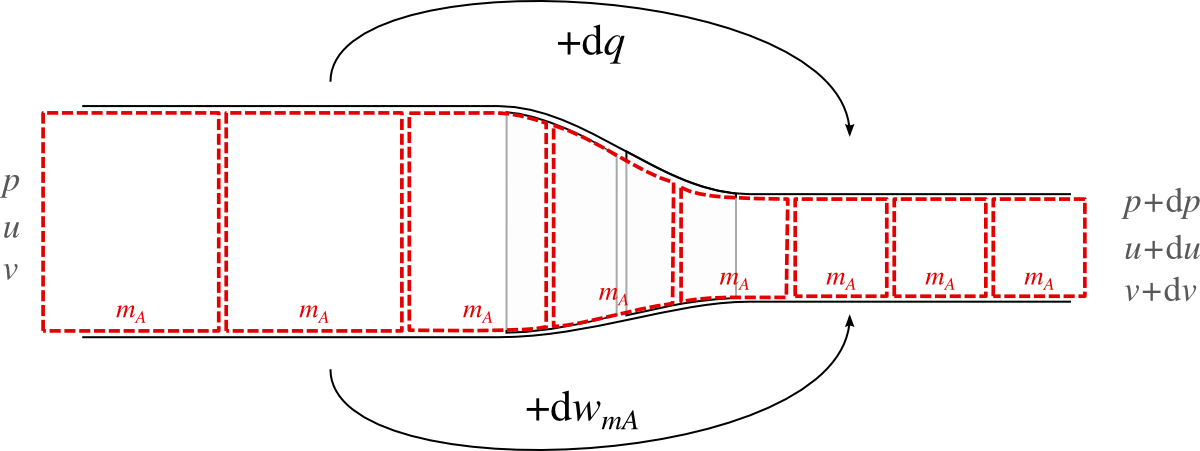
\includegraphics[width=\textwidth]{images/travail_sf_so1.png}
			\end{center}
			\supercaption{Une quantité de masse fixe $m_\A$ circule de gauche à droite à travers un compresseur. Elle est comprimée : ses propriétés passent de $p$ et $v$ à $p + \diff p$ et $v + \diff v$. Si on se place du point de vue d’un système fermé en transit, le transfert de travail est $\diff w_{m_\A} = - p \diff v$.}{schéma \cczero \oc}
			\label{fig_travail_so_vu_de_sf}
		\end{figure}

		Maintenant, observons le déroulement de ce \emph{même} phénomène du point de vue d’un système ouvert (\cref{fig_travail_so_vu_de_so}). Quelle puissance spécifique $\diff w_\text{S.0.}$ faut-il donner au compresseur pour que chaque particule de fluide reçoive un travail~$\diff w_{m_\A}$ ?

		\begin{figure}
			\begin{center}
				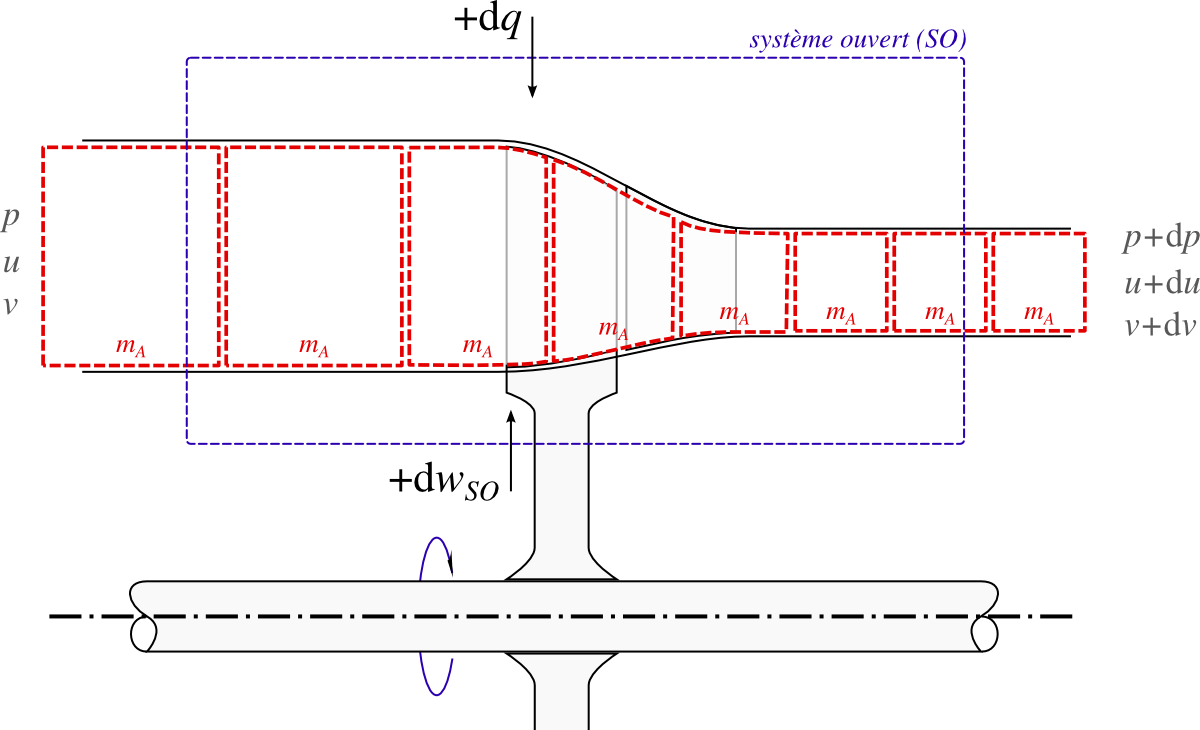
\includegraphics[width=\textwidth]{images/travail_sf_so2.png}
			\end{center}
			\supercaption{Le même écoulement qu’en \cref{fig_travail_so_vu_de_sf} observé du point de vue d’un système ouvert immobile traversé de gauche à droite par un flux continu. Nous cherchons à quantifier le travail $\diff w_\text{S.0.}$ à fournir au système pour que chaque quantité de masse $m_\A$ reçoive un travail $\diff w_{m_\A}$.}{schéma \cczero \oc}
			\label{fig_travail_so_vu_de_so}
		\end{figure}

		\clearfloats
		Le système ouvert a, lui, quatre transferts sous forme de travail :
	
		\begin{description}
			\item [La puissance spécifique d’insertion] $w_\text{insertion}$ (\ref{eq_puissance_spé_insertion}) est due à l’arrivée permanente du fluide à l’entrée du système. On a, du point de vue du système ouvert :
				\begin{equation}
					w_\text{insertion} = +p \ v
				\end{equation}

			\item [La puissance spécifique de compression] $-\diff w_{m_\A}$ est le travail spécifique que le système ouvert doit transférer à chaque quantité de masse $m_A$ pour qu’elle soit effectivement comprimée :
				\begin{equation}
					-\diff w_{m_\A} = -(-p \diff v)
					\label{eq_travail_so_wma}
				\end{equation}
		
			\item [La puissance spécifique d’extraction] $w_\text{extraction}$ est dépensée par le système ouvert pour faire sortir continûment le fluide.
		
				À la sortie, les propriétés du fluide sont devenues $p + \diff p$ pour la pression, et $v + \diff v$ pour le volume. On a ainsi :
				\begin{equation}
					w_\text{extraction} = -(p + \diff p) (v + \diff v)
				\end{equation}
				
			\item [La puissance spécifique reçue de l’extérieur] $\diff w_\text{S.O.}$ est la puissance qui alimente la compression : c’est la grandeur que nous souhaitons quantifier.

		\end{description}

		Ces quatre puissances s’annulent, car le transfert total de travail en jeu dans l’écoulement ne dépend pas du point de vue adopté :
		\begin{equation}
			\diff w_\text{S.0.} + w_\text{insertion} + (-\diff w_{mA}) + w_\text{extraction} = 0
		\end{equation}

		On peut donc quantifier la puissance spécifique $\diff w_\text{S.0.}$ qu’il faut donner au compresseur :
		\begin{IEEEeqnarray*}{rCl}
			\diff w_\text{S.0.} 	& = & - w_\text{insertion} + \diff w_{mA} - w_\text{extraction} \\
			\diff w_\text{S.0.} 	& = & -p \ v + (-p \diff v) + (p + \diff p) (v + \diff v) \\
					& = & -p \ v - p \diff v + p \ v + p\diff v + \diff p \ v + \diff p \ \diff v \\
					& = & \diff p \ v + \diff p \ \diff v
		\end{IEEEeqnarray*}

		Et comme le multiple $\diff p \times \diff v$ tend vers zéro lorsque nous utilisons des quantités infinitésimales, nous obtenons l’expression surprenante :
		\begin{equation}
			\diff w_\text{S.0.} = v \diff p
			\label{eq_travail_vdp}
		\end{equation}

		Les termes $\diff p$ et $\diff v$ dans notre étude ne sont pas nécessairement positifs : cette expression s’applique aussi bien dans les détentes que dans les compressions, tant qu’elles sont réversibles.
	
		En intégrant cette expression \ref{eq_travail_vdp} pour l’appliquer au cas général en régime continu, nous obtenons :
		\begin{IEEEeqnarray}{rCl}
			w_\text{S.0.} 			& = & \int v \diff p 					\label{eq_travail_w_rév_so} \\
			\dot{W}_\fromatob 	& = & \dot{m} \int_\A^\B v \diff p	\label{eq_travail_W_rév_so}
		\end{IEEEeqnarray}
		\begin{equationterms}
			\item lors d’un écoulement en régime continu,
			\item lorsque l’évolution est réversible,
			\item et quel que soit l’apport de chaleur.
		\end{equationterms}

		Ainsi, lorsque nous voulons quantifier le travail réversible dans un système ouvert, c’est l’intégrale $+\int v \diff p$, et non pas $-\int p \diff v$, qu’il nous faut calculer.
		
		Sur un diagramme pression-volume, nous pouvons visualiser ce travail en ajoutant le travail d’insertion et le travail d’extraction au travail de compression, comme montré en \cref{p-v_travail_so_construction}.

		\begin{figure}
			\begin{center}
				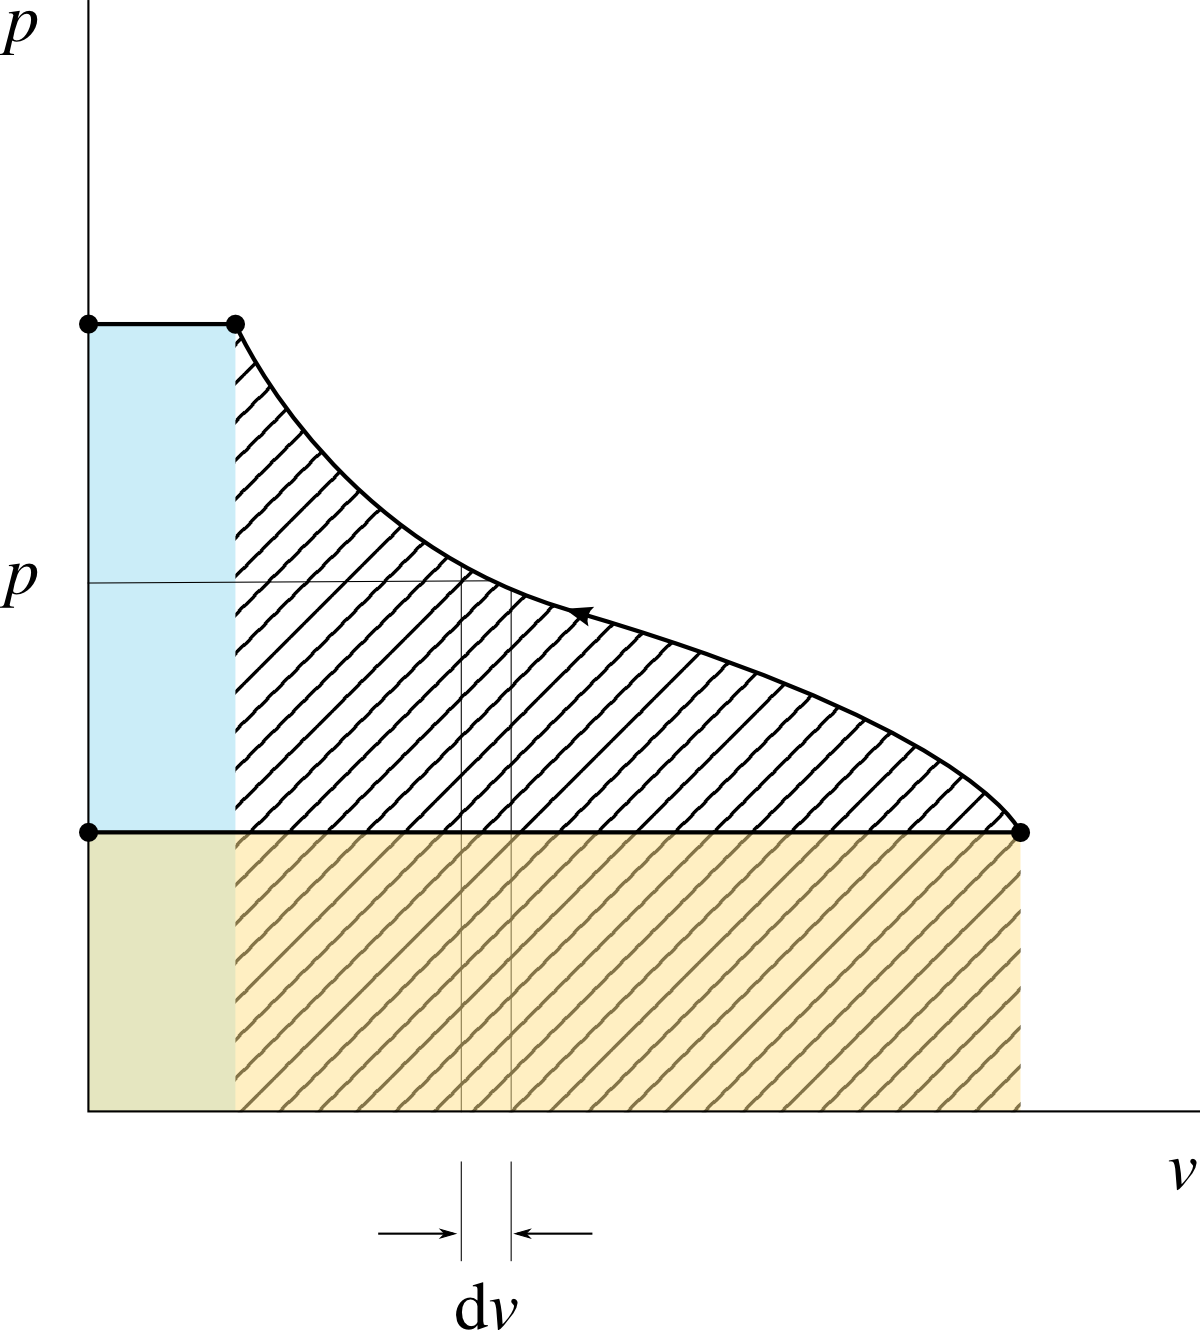
\includegraphics[width=8cm]{images/pv_systeme_ouvert_construction.png}
			\end{center}
			\supercaption{Travail reçu par un système ouvert traversé par un fluide, pendant une évolution lente.\\
			Le système reçoit d’abord le travail d’insertion ($p_\text{ini.} v_\text{ini.}$, en orange, positif) pour pénétrer dans le système,
			puis il dépense un travail de compression (aire hachurée, négative),
			et enfin il dépense le travail d’extraction ($p_\text{fin} v_\text{fin.}$, en bleu, négative).\\
			La somme nette de ces trois aires est la puissance spécifique à fournir au système ouvert.}{schéma \cczero \oc}
			\label{p-v_travail_so_construction}
		\end{figure}

		Un travail réversible effectué en régime continu se visualise donc par l’aire incluse \textit{à gauche} de la courbe, comme montré en \cref{p-v_travail_so}.

		\begin{figure}
			\begin{center}
				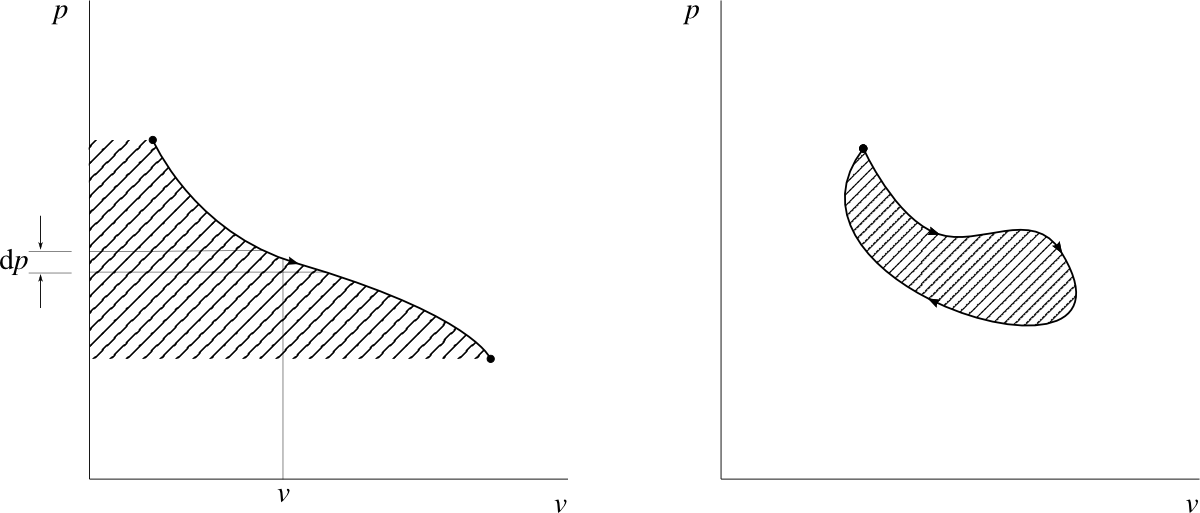
\includegraphics[width=\textwidth]{images/pv_systeme_ouvert.png}
			\end{center}
			\supercaption{Travail mesuré dans un système ouvert, pendant une évolution réversible.\\
			L’intégrale de $v \diff p$ est visualisée par l’aire à gauche de la courbe. \\
			Si le fluide revient à son état initial (ayant effectué un \vocab[cycle!thermodynamique]{cycle}), le travail développé est visualisé par l’aire incluse dans la courbe. Dans ce cas, la quantification est identique en système fermé et ouvert.}{schéma \cczero \oc}
			\label{p-v_travail_so}
		\end{figure}

		\begin{anexample}
			Une pompe à liquide compresse lentement un débit d’eau de~\SI{2}{\kilogram\per\second} depuis \SI{1}{\bar} jusqu’à \SI{20}{\bar}. Pendant la compression, le volume spécifique de l’eau reste constant à $v_L = \SI{e-3}{\metre\cubed\per\kilogram}$. Quelle est la puissance consommée sous forme de travail ?
				\begin{answer}
					Sur un diagramme pression-volume et de façon qualitative (c’est-à-dire sans représenter les valeurs numériques), l’évolution peut être représentée~ainsi :
							\begin{center}
								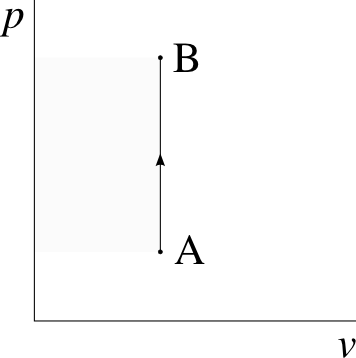
\includegraphics[width=3cm]{images/exe_pv_isochore_so.png}
							\end{center}
					Nous utilisons l’\cref{eq_travail_W_rév_so} en prenant garde aux unités. Comme $v$ est indépendant de $p$, l’intégration se fait sans peine : $\dot{W}_\fromatob 	= \dot{m} \int_\A^\B v \diff p = \dot{m} \ v_L \int_\A^\B \diff p = \dot{m} \ v_L \left[p\right]_{p_\A}^{p_\B} = 2 \times \num{e-3} \left(\num{20e5} - \num{1e5}\right) = \SI{+3,8e3}{\watt} = \SI{+3,8}{\kilo\watt}$.
				\end{answer}
					\begin{remark}Cette puissance est bien positive : c’est le fluide dans le système qui reçoit du travail.\end{remark}
					\begin{remark}Ici le volume spécifique $v_L$ est constant (comme toujours avec l’eau liquide). Si c’était la pression qui était constante, alors le travail serait nul même si $v$ était amené à varier.\end{remark}
		\end{anexample}
		
		\begin{anexample}
			Un compresseur compresse lentement un débit d’air de~\SI{2}{\kilogram\per\second} depuis \SI{1}{\bar} jusqu’à \SI{20}{\bar}. Pendant la compression, le volume spécifique et la pression de l’air sont liés par la relation $p \ v^{\num{1,35}} = k$. À l’entrée, le volume spécifique de l’air est de $v_\A = \SI{0,8}{\metre\cubed\per\kilogram}$.\\
			Quelle est la puissance consommée sous forme de travail ?
				\begin{answer}
				Sur un diagramme pression-volume et de façon qualitative, l’évolution peut être représentée ainsi :
							\begin{center}
								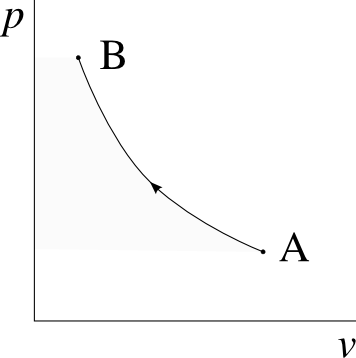
\includegraphics[width=3cm]{images/exe_pv_exp_so.png}
							\end{center}
					Ici le volume spécifique est fonction de la pression : nous avons $v = \left(\frac{k}{p}\right)^{\frac{1}{\num{1,35}}} = k^{\frac{1}{\num{1,35}}} p^{-\frac{1}{\num{1,35}}}$.\\
					Nous partons de l’\cref{eq_travail_W_rév_so} : \\
					$\dot{W}_\fromatob
					= \dot{m} \int_\A^\B v \diff p
					= \dot{m} \ k^{\frac{1}{\num{1,35}}} \int_\A^\B p^{-\frac{1}{\num{1,35}}} \diff p\\
					= \dot{m} \ k^{\frac{1}{\num{1,35}}} \left[\frac{1}{-\frac{1}{\num{1,35}} +1} p^{-\frac{1}{\num{1,35}} +1}\right]_{p_\A}^{p_\B}
					= \dot{m} \ \left(p_\A v_\A^{\num{1,35}}\right)^{\frac{1}{\num{1,35}}} \frac{1}{\num{0,25926}} \left[p^{\num{0,25926}}\right]_{p_\A}^{p_\B}
					= 2 \left(\num{20e5} \times \num{0,8}^{\num{1,35}}\right)^{\frac{1}{\num{1,35}}} \frac{1}{\num{0,25926}} \left[\left(\num{20e5}\right)^{\num{0,25926}} - \left(\num{1e5}\right)^{\num{0,25926}}\right]
					= \SI{+6,666e6}{\watt} = \SI{+6,666}{\mega\watt}$.
				\end{answer}
					\begin{remark}Ici la clé est de bien décrire la fonction $v_{(p)}$ avant de procéder à l’intégration.\end{remark}
					\begin{remark}La puissance du compresseur est \num{1700} fois plus grande que celle de la pompe de l’exemple précédente. De plus, le volume spécifique de l’air à l’entrée est \num{800} fois plus grand : il faudra une machine de taille beaucoup plus importante (elle doit absorber un débit volumique $\dot{V}_\A = \dot{m} \ v_\A = \SI{1,6}{\metre\cubed\per\second} = \SI{1600}{\liter\per\second}$ à l’entrée).\end{remark}
		\end{anexample}


	\subsection{Travail d’un fluide en évolution rapide}
	\index{travail!en système ouvert, en évolution rapide}\index{travail!transferts irréversibles}\index{système!ouvert, travail en évolution rapide}
	
	
		Lorsque le fluide évolue de façon rapide (ce qui est toujours le cas en pratique), nous retrouvons les phénomènes que nous avons décrits au chapitre précédent (\S\ref{ch_évolutions_irr_sf}) : la pression exercée sur les parois mobiles ne correspond plus à la pression «~moyenne~» à l’intérieur du fluide. Le travail à fournir dans les compressions est plus grand et le travail réceptionné pendant les détentes est plus faible que lors des évolutions lentes.
		
		Le fait d’utiliser un système ouvert pour comptabiliser les transferts d’énergie ne change bien sûr rien au problème. Nous n’avons pas les moyens de prédire analytiquement le travail à fournir pour une compression à une vitesse donnée. Le problème –calculer la distribution spatiale de la pression à l’intérieur du fluide en fonction du temps– relève de la mécanique des fluides, et sera quoi qu’il en soit résolu au cas-par-cas.
		
		Sur nos diagrammes pression-volume, nous représentons les évolutions irréversibles avec un trait en pointillés, pour bien les différencier des évolutions réversibles (\cref{fig_pv_evolution_irr_so}).
		
		\onlyframabook{\begin{figure}[htc]}%handmade
		\onlyamphibook{\begin{figure}}
			\begin{center}
				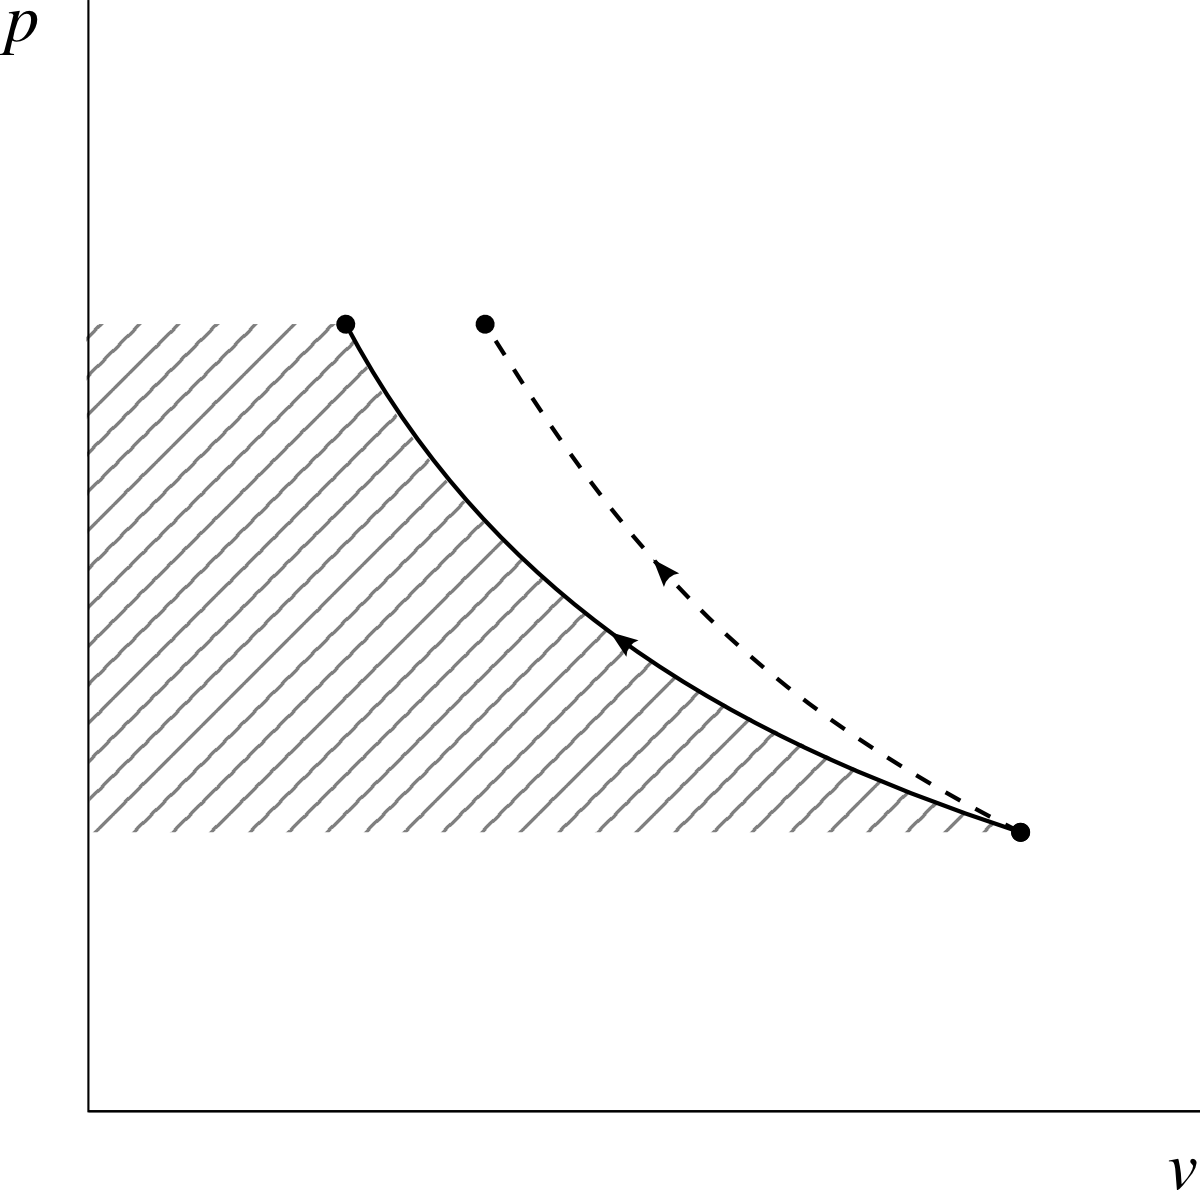
\includegraphics[width=8cm]{images/pv_compression_irreversible_so.png}
			\end{center}
			\supercaption{Compressions réversible (trait continu) et irréversible (en pointillés) représentées sur un diagramme pression-volume. Dans un système ouvert, les transferts de travail peuvent être visualisés avec l’aire à gauche de la courbe, mais uniquement lorsque les évolutions sont réversibles.}{schéma \cczero \oc}
			\label{fig_pv_evolution_irr_so}
		\end{figure}
	
		\clearfloats %handmade
		\begin{anexample}\index{adiabatiques!irréversibles, évolutions}\index{chaleur!transformation de travail en}\index{travail!transformation en chaleur}
			De l’air est compressé en continu de 1 à~\SI{20}{\bar} dans un compresseur. Dès la sortie du compresseur l’air rentre dans une turbine qui le détend de 20 à~\SI{1}{\bar}. Dès la sortie de la turbine, l’air est à nouveau inséré dans le compresseur.
			
			Quelle sera l’allure des évolutions sur un diagramme pression-volume ?
					\begin{answer}
						Si les évolutions se font lentement, la pression et le volume spécifique passent toujours par les mêmes valeurs pendant les allers-retours :
							\begin{center}
								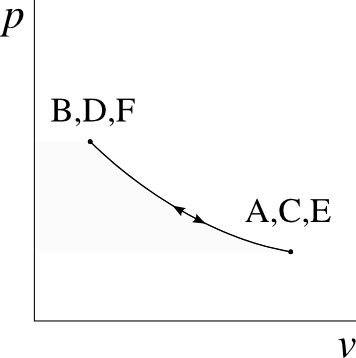
\includegraphics[height=3cm]{images/exe_pv_rev_so.png}
							\end{center}
						En revanche, si les évolutions sont rapides, à chaque trajet le volume spécifique final est plus grand que ce qu’il aurait été pendant un trajet lent :
							\begin{center}
								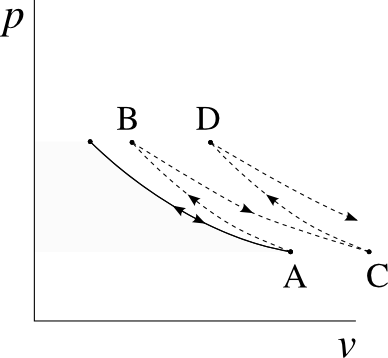
\includegraphics[height=3cm]{images/exe_pv_irr_so.png}
							\end{center}
						Ainsi, les propriétés se décalent progressivement sur le diagramme pression-volume. Si les évolutions ne se font pas lentement, le compresseur demande plus d’énergie que la turbine est capable de prélever au retour. Cet excédent d’énergie est absorbé par l’air, ce qui augmente son énergie interne et sa température.
					\end{answer}

		\end{anexample}
	
\section{Quantifier la chaleur avec un système ouvert}
\index{chaleur!calcul en système ouvert}\index{système!ouvert, calcul de chaleur}

	Avec un système ouvert nous allons utiliser la même méthode qu’avec un système fermé : comme nous ne savons pas quantifier les transferts de chaleur directement, nous allons toujours procéder par déduction.
	Mathématiquement, nous ne faisons que réutiliser l’\cref{eq_grande_sfee_deltas_h} pour obtenir :
	\begin{IEEEeqnarray}{rCl}
		\dot{Q}_{1 \to 2} & = & \dot{m} \left( \Delta h + \Delta e_\text{méca.}\right) - \dot{W}_{1 \to 2} \\
			q_{1 \to 2} 	& = & \Delta h + \Delta e_\text{méca.}  - w_{1 \to 2}
	\end{IEEEeqnarray}
	\begin{equationterms}
		\item pour un système ouvert.
	\end{equationterms}
		
		Là encore, toute la difficulté pour quantifier un transfert de chaleur est de prédire et quantifier le changement de l’enthalpie, $\Delta h$. Pour les gaz, $h$ est quasiment proportionnelle à la température ; pour les liquides et vapeurs, la relation est plus complexe. Nous apprendrons à quantifier l’enthalpie dans les fluides aux \coursquatre et \courscinq.
\index{système!ouvert|)textbf}
